\documentclass[dvipsnames]{beamer}
\usepackage[utf8]{inputenc}
\usepackage{beamerthemeCourse}
\usepackage[absolute,overlay]{textpos}
\usepackage{listings}
\usepackage[utf8]{inputenc}

\usepackage{./beamerthemeCourse}
\usepackage{listings}
\lstset{language = Tex}

\usepackage[absolute,overlay]{textpos}
\usepackage[normalem]{ulem}
\usepackage{numprint}       % Histoire que les chiffres soient bien

\usepackage{amsmath}        % La base pour les maths
\usepackage{amsthm}
\usepackage{mathrsfs}       % Quelques symboles supplémentaires
\usepackage{amssymb}        % encore des symboles.
\usepackage{amsfonts}       % Des fontes, eg pour \mathbb.
\usepackage{rotating}

% ---- IMPOSTAZIONI PACCHETTI ----
\definecolor{forestgreen}{rgb}{0.13, 0.55, 0.13}
\definecolor{mypink}{rgb}{0.858, 0.188, 0.478}

\lstset{
    language=[LaTeX]Tex,%C++,
    keywordstyle=\color{blue}, %\bfseries,
    basicstyle=\small\ttfamily,
    commentstyle=\color{forestgreen}\ttfamily,
    stringstyle=\rmfamily,
    numbers=left,%
    numberstyle=\scriptsize, %\tiny
    stepnumber=1,
    numbersep=8pt,
    showstringspaces=false,
    breaklines=true,
    frameround=ftff,
    frame=single
}
\title{Tipologie di documenti}
\subtitle{Divisione del documento e le varie tipologie}
\author{F.Fasolato, G.Zecchin, Guido Male, A.Bari}
\date{AA 2018-2019}

\newcommand{\mbook}{\textbf{\textcolor{mypink}{book}}}
\newcommand{\marticle}{\textbf{\textcolor{blue}{article}}}
\newcommand{\mreport}{\textbf{\textcolor{forestgreen}{report}}}

\begin{document}

    \maketitle
    \begin{frame}{Outline}
        \tableofcontents
    \end{frame}
    

\section{Tabelle Semplici}
\begin{frame}

  \frametitle{Tabelle Semplici}
  
  \begin{itemize}
   \item Si inizializzano come gli elenchi puntati
   \begin{itemize}
    \item Vedremo dopo che ci sono delle aggiunte da fare...
   \end{itemize}
   \item Dobbiamo specificare la loro posizione nel testo
   \item Sono abbastanza intuitive da fare
  \end{itemize}
  

\end{frame}

\begin{frame}
 \frametitle{Personalizzazione}
 
 Gli elenchi possono essere personalizzati a piacimento!
 \begin{itemize}
  \item[-]<1-> possiamo inserire
  \item[/]<2-> il simbolo
  \item[.]<3-> che più ci piace!
 \end{itemize}

\end{frame}

\begin{frame}[fragile]
 \frametitle{Personalizzazione - 2}
 
Per far ciò bisogna utilizzare la seguente sintassi:
 
\begin{block}{Esempio: Una lista puntata personalizzata}
\begin{code}
\begin{minted}[linenos]{latex}
\begin{itemize}
 \item[-] Primo
 \item[/] Secondo
 \item[.] Quinto?!?!?
\end{itemize}
\end{minted}
\end{code}
\end{block}
 
Possiamo mettere ciò che vogliamo, anche frasi intere. Però 
attenzione che parole troppo lunghe provocano effetti indesiderati.
\end{frame}

\begin{frame}
 \frametitle{Personalizzazione - 3}
 
 \begin{itemize}
  % Intenzionale
  \item[parole troppo lunghe] potrebbero rompere la formattazione!
 \end{itemize}

  
 \begin{textblock*}{5cm}(7cm,5.5cm)
   
\includegraphics{broken}
 \end{textblock*}
\end{frame}

\section{Apici, pedici, sommatoria, produttoria \dots}
  \begin{frame}{Apici, pedici, sommatoria, produttoria \dots}
    
    \begin{itemize}
      \item<1-> Esponenti: $a^2$
      \item<2-> Pedici: $a_1$
      \item<3-> Apici: $a^{*}$
      \item<4-> Sommatoria: $\sum_{i=1}^n a_i$
      \item<5-> Produttoria: $\prod_{i=1}^n a_i$
      \item<6-> Frazione: $\frac{x + 1}{x + 2}$
      \item<7-> Radice quadrata: $\sqrt{a^2 + b^2}$
    \end{itemize}

\end{frame}

\begin{frame}
 
 \begin{figure}
  \centering
  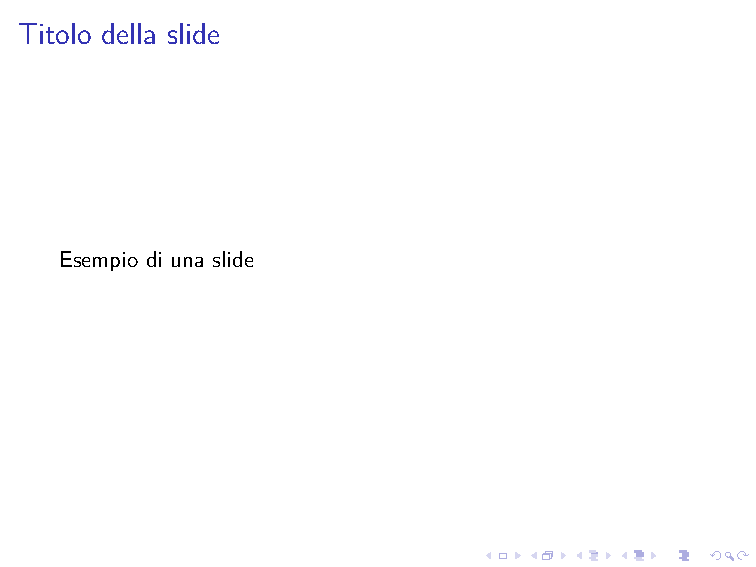
\includegraphics[scale=0.70]{esempio}
 \end{figure}

\end{frame}

\begin{frame}
 
 \frametitle{Un po' deludente...}
 
 \begin{itemize}
  \item<1-> Manca il tema! \texttt{\textbackslash usetheme\{ \}}
  \item<2-> Manca il titolo! \texttt{\textbackslash title\{ \}}
  \item<3-> Mancano gli autori! \texttt{\textbackslash author\{ \}}
  \item<4-> E vogliamo mettere l'istituto?? \texttt{\textbackslash institute\{ 
\}}
  \item<5-> Potremmo mettere anche la data della presentazione dato che ci 
siamo... 
\texttt{\textbackslash date\{ \}}
 \end{itemize}
 
 Abbelliamo un attimo il nostro esempio!
 
 \begin{textblock*}{4cm}(8cm,6cm)
    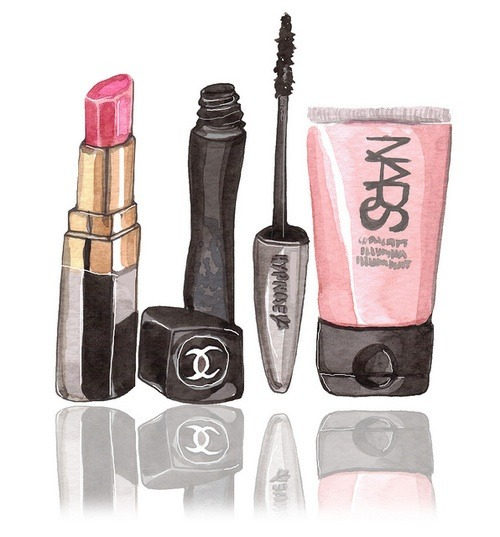
\includegraphics[scale=0.10]{beauty}
 \end{textblock*}
 
 
 \begin{textblock*}{5cm}(7cm,2cm)
    
\includegraphics[scale=0.60]{lack}
 \end{textblock*}

\end{frame}
 

\begin{frame}[fragile]
 \frametitle{Riproviamo!}
 
 Proviamo con questo esempio:
\begin{esempio}{Nuovo codice}
    \codedInput{res/examples/beamertema.tex}
\end{esempio}
\end{frame}

\begin{frame}
 
 \frametitle{E il risultato è...}
 
 \begin{figure}[h]
  \centering
  
\includegraphics[scale=0.68]{beamer_theme}
  \label{img:maketitle}
 \end{figure}
 
\end{frame}

\begin{frame}
 \frametitle{Orientare le pagine - 2}
 
 Si può:
 \begin{itemize}
  \item<1-> Ruotare una sola pagina con il pacchetto \texttt{pdflscape}
  \item<2-> Ruotare tutto il documento con l'opzione \texttt{landscape} quando 
creiamo un nuovo documento
 \end{itemize}

 
%  \begin{textblock*}{5cm}(7.5cm,1.1cm)
%   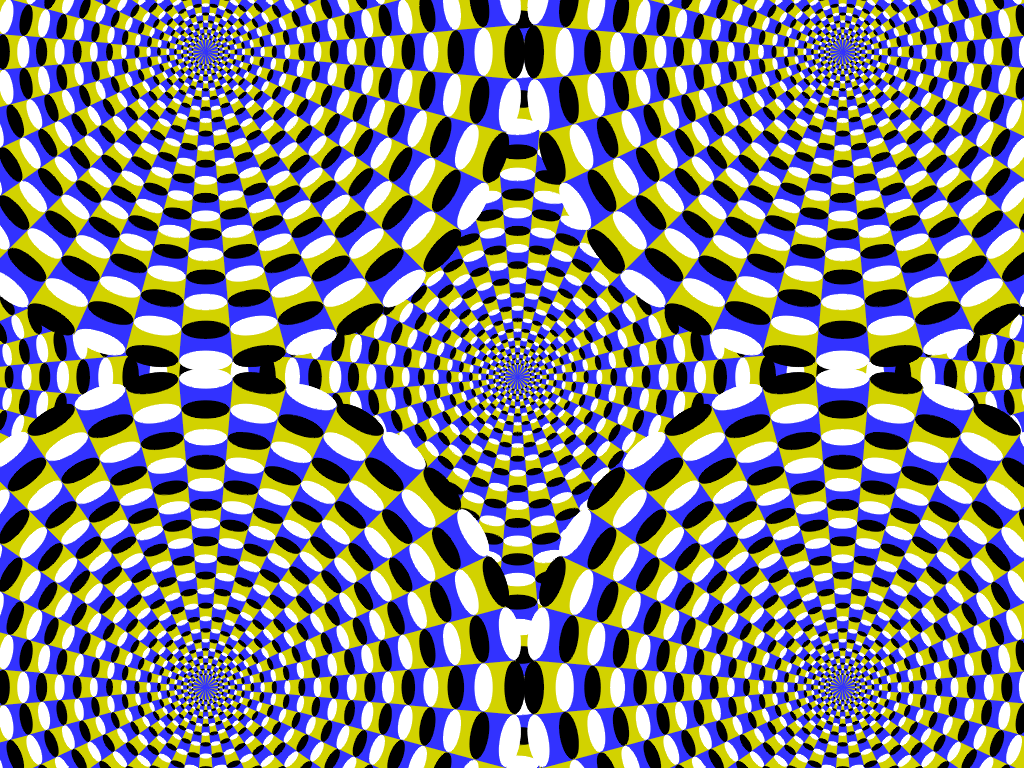
\includegraphics[scale=0.12]{spiral}
%  \end{textblock*}
 
%  \begin{textblock*}{5cm}(3cm,6cm)
%   
\includegraphics[scale=0.05]{recycle}
%  \end{textblock*}
\end{frame}

\section{Funzioni e insiemi}
  \begin{frame}{Funzioni e insiemi}

	Definizione di funzione

	Si usano i comandi \mintinline{latex}{\colon} (per i due punti), \mintinline{latex}{\to} e \mintinline{latex}{\mapsto}

    \begin{esempio}{Funzione identità}
	  \centering
	  $f \colon \mathbb{R} \to \mathbb{R}$ \\
	  $x \mapsto x$
    \end{esempio}

	Gli insiemi principali:

	\begin{table}[h!]
	\begin{tabular}{l l}
	\hline
	$\mathbb{N}$ \mintinline{latex}{\mathbb\{N\}} & $\mathbb{Z}$ \mintinline{latex}{\mathbb\{Z\}} \\
	$\mathbb{Q}$ \mintinline{latex}{\mathbb\{Q\}} & $\mathbb{R}$ \mintinline{latex}{\mathbb\{R\}} \\
	\hline
	\end{tabular}
	\end{table}

\end{frame}

\section{Enunciati}
  \begin{frame}{Definizioni, Teoremi, Corollari}

	Un enunciato in Latex ha bisogno di:

    \begin{itemize}
      \item un tipo/stile (ad esempio definizioni e teoremi)
      \item un nome (Definizione o Teorema)
	  \item un titolo
    \end{itemize}

	Il comando \mintinline{latex}{\newtheorem} \{nome dell'enunciato\} \{titolo\} [sezione] per definire enunciati \textbf{va dichiarato nel preambolo}.

\end{frame}

\begin{frame}[fragile]
\frametitle{Unit\`a di misura}

\begin{table}[]
\caption{Unit\`a di misura in \LaTeX}
\begin{tabular}{l|llll}
\cline{1-2}
pt & Punto, ovvero 0.3515 mm  \\ \cline{1-2}
mm &  Millimetro  \\ \cline{1-2}
cm &  Centimetro  \\ \cline{1-2}
in &  Pollice  \\ \cline{1-2}
ex &  Altezza della "x" minuscola nel font corrente \\ \cline{1-2}
em &  Altezza della "M" maiuscola nel font corrente \\ \cline{1-2}
mu &  Math Unit, ovvero 1/18 em  \\ \cline{1-2}
\end{tabular}
\end{table}

\end{frame}


\begin{frame}[fragile]
\frametitle{Lengths - 1}

Le Lengths sono delle unit\`a di misura della distanza relativa di alcuni elementi che costituiscono il documento. Hanno gi\`a valori di default, ma nel caso si necessiti di cambiarle, bisogna usare il comando:\newline

\mintinline{latex}{\setlength{\lengthname}{value_in_specified_unit}}\newline

Per esempio, la distanza fra le colonne di un documento "a due colonne" pu\`o essere fissata ad un Pollice con:\newline

\mintinline{latex}{\setlength{\columnsep}{1in}}

\end{frame}

\begin{frame}[fragile]
\frametitle{Lengths - 2}

\begin{table}[]
\caption{Tipologie di Lengths}
\begin{tabular}{l|llll}
\cline{1-2}
\mintinline{latex}{\baselineskip} & Distanza verticale fra due righe in un paragrafo  \\ \cline{1-2}
\mintinline{latex}{\columnsep} & Distanza orizzontale fra due colonne  \\ \cline{1-2}
\mintinline{latex}{\columnwidth} & Larghezza di una colonna  \\ \cline{1-2}
\mintinline{latex}{\linewidth} & Larghezza di una riga  \\ \cline{1-2}
\mintinline{latex}{\paperwidth} & Larghezza della pagina  \\ \cline{1-2}
\mintinline{latex}{\paperheight} & Altezza della pagina   \\ \cline{1-2}
\mintinline{latex}{\parindent} & Indentazione del paragrafo  \\ \cline{1-2}
\mintinline{latex}{\paperheight} & Altezza della pagina   \\ \cline{1-2}
\mintinline{latex}{\parskip} & Spazio verticale fra paragrafi   \\ \cline{1-2}
\mintinline{latex}{\textwidth} & Larghezza dell'area di testo nella pagina  \\ \cline{1-2}
\mintinline{latex}{\textheight} & Altezza dell'area di testo nella pagina   \\ \cline{1-2}
\end{tabular}
\end{table}

\end{frame}
\section{Enunciato di Murphy}
  \begin{frame}{Enunciato di Murphy}

	\begin{teoremaMurphy} Se qualcosa può andar male, lo farà \end{teoremaMurphy}
	\begin{corollarioMurphy} Preoccuparsi è inutile \end{corollarioMurphy}
	\begin{proof} Esperienze di vita \end{proof} %ambiente proof predefinito

	\begin{figure}[h!]
	
\includegraphics[scale=0.15]{murphy}
	\end{figure}

\end{frame}

\begin{frame}{Esempio}

    \begin{esempio}{Esempio di utilizzo}
    \begin{code}
      \inputminted[linenos, fontsize=\footnotesize] {latex} {res/snippets/example6.tex}
     \end{code}
    \end{esempio}

\end{frame}

\section{Ulteriori comandi \dots}
\begin{frame}{Ulteriori comandi \dots}

	Matrici inserendo il contenuto nei blocchi \textbf{pmatrix} e \textbf{bmatrix}: 

	\[
	\begin{pmatrix}
	1 & 2 \\
	3 & 4
	\end{pmatrix}
	\]

	\[
	\begin{bmatrix}
	1 \\
	2
	\end{bmatrix}
	\]

	Parentesi grandi con i comandi \mintinline{latex}{\Bigl} e \mintinline{latex}{\Bigr}  :

	\[
	\Bigl(1+\frac{1}{n}\Bigr)^n
	\]

\end{frame}

\begin{frame}{Comandi Specifici}

	\begin{table}[h!]
	\begin{tabular}{p{2.6cm} p{2.6cm} p{2.6cm}}
	\hline
	$<$ & $>$ & $\leq$ \mintinline{latex}{\leq} \\[0.4cm]
	$\geq$ \mintinline{latex}{\geq} & $\sim$ \mintinline{latex}{\sim} & $\simeq$ \mintinline{latex}{\simeq} \\[0.4cm]
	$\cong$ \mintinline{latex}{\cong} & $\equiv$ \mintinline{latex}{\equiv} & {}\\
	\hline
	\end{tabular}
	\end{table}

    In casi specifici conviene cercare quali simboli fanno al vostro caso in base alle necessità \dots

\end{frame}

\section{Esercizi}
\begin{frame}

  \frametitle{Esercizi}

  \begin{block}{Esercizio 1}
    Creare una presentazione che contenga il vostro nome, la data di oggi, il 
vostro dipartimento di appartenenza e ovviamente il titolo (come in 
Slide~\ref{img:maketitle}). Applicate un tema di quelli predefiniti al seguente 
link \url{https://hartwork.org/beamer-theme-matrix/} (usate 
\texttt{\textbackslash maketitle}).
  \end{block}

  \begin{block}{Esercizio 2}
    Aggiungete un paio di slide alla presentazione creata nell'Esercizio 1 
inserendo liste puntate/numerate e/o immagini su un argomento a vostra scelta 
(per esempio come fare una crostata).
  \end{block}
\end{frame}

\begin{frame}

  \frametitle{Esercizi - 2}
 
  \begin{block}{Esercizio 3}
    Inserire degli effetti a piacere tra le slide create nell'Esercizio 2 e 
impostare l'avanzamento automatico delle slide ogni 2 secondi.
  \end{block}
\end{frame}

\begin{frame}[fragile]

  \frametitle{Soluzioni - 1}
 
\begin{block}{Soluzione sercizio 1}
\lstinputlisting{res/examples/sol1}
\end{block}
\end{frame}

\begin{frame}[fragile]

  \frametitle{Soluzioni - 2}
  
\begin{block}{Soluzione esercizio 2 - parte 1}
\lstinputlisting{res/examples/sol2}
\end{block}
\end{frame}

\begin{frame}[fragile]

  \frametitle{Soluzioni - 3}
  
\begin{block}{Soluzione esercizio 2 - parte 2}
\lstinputlisting{res/examples/sol2-1}
\end{block}
\end{frame}

\begin{frame}[fragile]

  \frametitle{Soluzioni - 4}
  
\begin{block}{Soluzione esercizio 3 - parte 1}
\lstinputlisting{res/examples/sol3}
\end{block}
\end{frame}

\begin{frame}[fragile]

  \frametitle{Soluzioni - 5}
  
\begin{block}{Soluzione esercizio 3 - parte 2}
\lstinputlisting{res/examples/sol3-1}
\end{block}
\end{frame}

\end{document}
